\section{Auswertung}
\label{sec:Auswertung}

\subsection{Vorbereitung}
Bei der Vorbereitung wurde beim linken Schwingkreis eine Eigenfrequenz von $f_{\text{eigen}}=30.61 \si{\kilo\hertz}$ bei einer
Phasendifferenz von $\SI{0}{\degree}$ gemessen. 
Der verstellbare Kondensator wird so eingestellt, dass der rechte Schwingkreis die gleiche Eigenfrequenz hat, wie der linke.
Die Referenzwerte der Bauteile des benutzten Schltkastens sind in \autoref{tab:kasten_links} und \autoref{tab:kasten_rechts}.
Die Anzahl der Maxima, beziehungsweise Minima, sind in \autoref{tab:schwing_maxima} aufgeführt. Außerdem ist die 
Dauer einer Schwebung aufgetragen.

\begin{table}
  \centering
  \caption{Werte des linken Schaltkreises.}
  \label{tab:kasten_links}
  \begin{tabular}{c c c}
      \toprule
      {$L \:/\: \si{\milli\henry} $} & $C \:/\: \si{\nano\farad} $ & $C_{\text{Spule}}\:/\: \si{\nano\farad}$ \\
      \midrule
      32.351 & 0.8015 & 0.037 \\
      \bottomrule
  \end{tabular}
\end{table}

\begin{table}
  \centering
  \caption{Werte des rechten Schaltkreises.}
  \label{tab:kasten_rechts}
  \begin{tabular}{c c c}
      \toprule
      {$L \:/\: \si{\milli\henry} $} & $C \:/\: \si{\nano\farad} $ & $C_{\text{Spule}}\:/\: \si{\nano\farad}$ \\
      \midrule
      23.954 & 0.7932 & 0.028 \\
      \bottomrule
  \end{tabular}
\end{table}

\begin{table}
  \centering
  \caption{Anzahl Maxima der Schwebung.}
  \label{tab:schwing_maxima}
  \begin{tabular}{c c c}
      \toprule
      {$C_K \:/\: \si{\nano\farad}$} & Schwingungsmaxima & $\Delta t\:/\: \si{\micro\second}$ \\
      \midrule
      9.99  & 13 & 235 \\ 
      8.00  & 11 & 195 \\ 
      6.47  & 10 & 155 \\ 
      5.02 & 8 & 125 \\ 
      4.00 & 7 & 100 \\
      3.00 & 6 & 75 \\
      2.03 & 4 & 50\\ 
      \bottomrule
  \end{tabular}
\end{table}

\subsection{Fundamentalschwingung}
Im folgenden werden die beiden Fundamentalschwingungen in Abhängigkeit der Kopplungskapazität $C_{\text{K}}$ des Kopplungskondensators
bestimmt. 


\begin{table}
  \centering
  \caption{Fundamentalschwingungen}
  \label{tab:aufgabeC}
  \begin{tabular}{c c c c c c}
      \toprule
      {$f_+\;/ \si{\kilo\hertz}$} & {$f_-\;/ \si{\kilo\hertz}$} & {$V_1 \:/\: \si{\milli\volt}$} & {$V_2 \:/\: \si{\milli\volt}$} & {$C_K \:/\: \si{\nano\farad}$} & $I_2 \:/\:\si{\milli\ampere}$ \\
      \midrule
      38 & 49 & 60 & 110 & 9.99 & 1.22 \\
      40 & 50 & 55 & 110 & 8.00 & 1.51 \\
      40 & 50 & 55 & 110 & 6.47 & 1.87 \\
      38 & 55 & 50 & 110 & 5.02 & 2.42 \\
      40 & 58 & 50 & 105 & 4.00 & 2.90 \\
      40 & 62 & 50 & 105 & 3.00 & 3.86 \\
      40 & 73 & 50 & 100 & 2.03 & 5.44 \\
      40 & 76 & 55 & 95 & 1.01 & 10.39 \\
      \bottomrule
  \end{tabular}
\end{table}


\begin{figure}
  \centering
  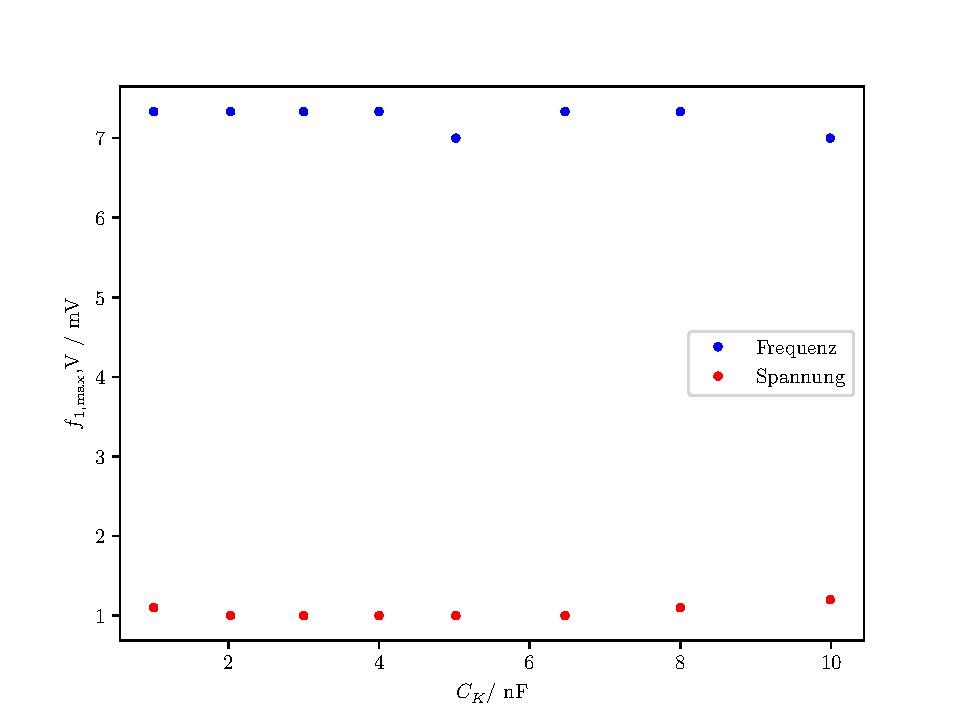
\includegraphics{freq1.pdf}
  \caption{Die aufgenommenen Messwerte}
  \label{fig:freq1}
\end{figure}

\begin{figure}
  \centering
  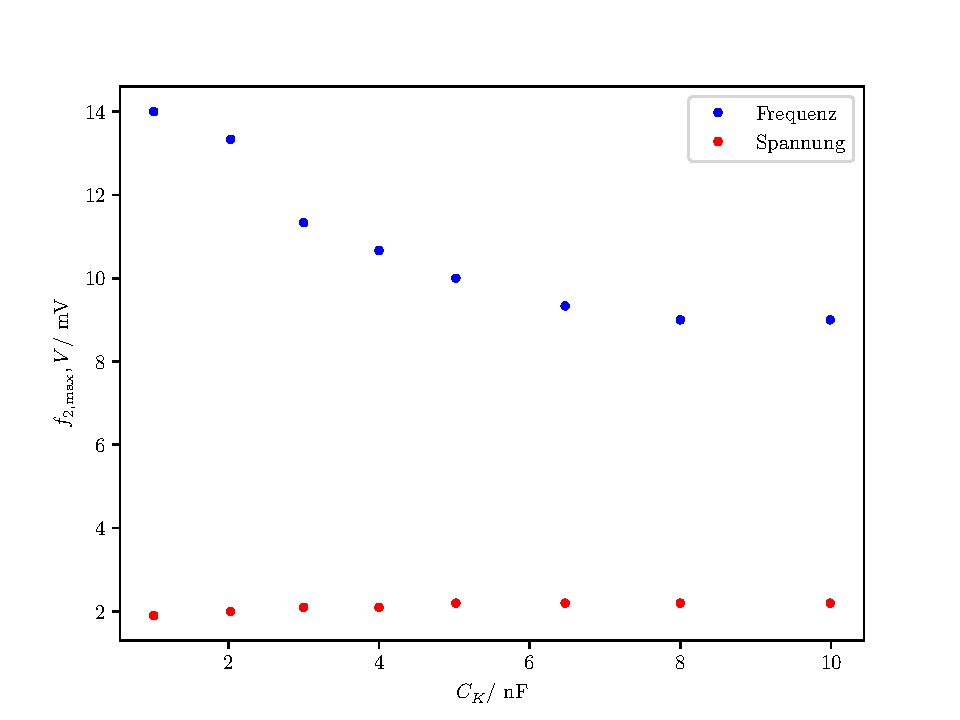
\includegraphics{freq2.pdf}
  \caption{Die aufgenommenen Messwerte}
  \label{fig:freq2}
\end{figure}


% \I_2  = \frac{U}{R\sqrt{4 + \frac{R^2C_K^2}{LC}(1 + \frac{C}{C_K}})}
Der Strom $I_2$ wird mithilfe des Widerstandes $R=48\Omega$ berechnet.
Die Frequenz der ersten Fundamentalschwingung berechnet sich durch %Formel in Theorie angeben und dann nur zitieren?
$f_+ = \frac{1}{2\pi\sqrt{LC}}$ 

und die der zweiten Fundamentalschwingung durch 
$f_- = \frac{1}{2\pi\sqrt{L\frac{CC_K}{2C+C_K}}}$. 

Es werden die geringen Kapazitäten der beiden Spulen ebenfalls berücksichtigt, wodurch sich die Frequenzen ergeben zu
$f_+ = \frac{1}{2\pi\sqrt{L(C + C_\text{Sp})}}$ und $f_- = \frac{1}{2\pi\sqrt{L\Bigl(\dfrac{CC_K}{2C+C_K} + C_\text{Sp}\Bigr)}}$. 

Der theoretisch zu erwartende Wert für den Strom $I_2$ berechnet sich durch EINE FORMEL. 

%Ich weiß nicht genau, was die Formel von I_2aussagt, ich warte einfach auf deine Theorie

\begin{table}
  \centering
  \caption{Die erwarteten Theoriewerte.}
  \label{tab:theorietabelle}
  \begin{tabular}{c c c c c c c}
      \toprule
      $f_+ \:/\: \si{\kilo\hertz}$ & $f_{+, \text{theo}} \:/\: \si{\kilo\hertz}$ & $f_- \:/\: \si{\kilo\hertz}$ & $f_{-, \text{theo}} \:/\: \si{\kilo\hertz}$ & $C_K \:/\: \si{\nano\farad}$ & $I_2 \:/\: \si{\milli\ampere}$ & $I_{2,\text{theo}} \:/\: \si{\milli\ampere}$ \\
      \midrule
      38 & 35.32 & 49 & 32.80 & 9.99 & 1.22 & 1 \\
      40 & 35.32 & 50 & 33.33 & 8.00 & 1.51 & 1 \\
      40 & 35.32 & 50 & 33.95 & 6.47 & 1.87 & 1 \\
      38 & 35.32 & 55 & 34.85 & 5.02 & 2.42 & 1 \\
      40 & 35.32 & 58 & 35.85 & 4.00 & 2.90 & 1 \\
      40 & 35.32 & 62 & 37.41 & 3.00 & 3.86 & 1 \\
      40 & 35.32 & 73 & 40.19 & 2.03 & 5.44 & 1 \\
      40 & 35.32 & 76 & 47.52 & 1.01 & 10.39 & 1 \\
      \bottomrule
  \end{tabular}
\end{table}

\pagebreak